\documentclass{standalone}
\renewcommand{\familydefault}{\sfdefault}

\usepackage{tikz}
\usetikzlibrary{calc}

\begin{document}
\scalebox{2.8}{
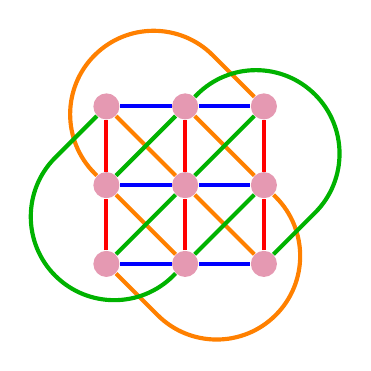
\begin{tikzpicture}
  \clip (-1, -1) rectangle (3, 3);

  \foreach \x in {0,1,2}
    \foreach \y in {0,1,2}
    {
      \node [fill=purple!40!white, circle] (P-\x-\y) at (\x, \y) {};
    }

  \foreach \z in {0,1,2}
  {
    \draw [line width=1.5, red] (P-\z-0) -- (P-\z-1) -- (P-\z-2);
    \draw [line width=1.5, blue] (P-0-\z) -- (P-1-\z) -- (P-2-\z);
  }

  \draw [line width=1.5, orange] (P-0-2) -- (P-1-1) -- (P-2-0);
  \draw [line width=1.5, orange] (P-1-0) --
                                 (P-0-1) --
				 ($(P-0-1) + (-0.15, 0.15)$) arc(225:45:{0.75*sqrt(2)}) --
                                 (P-2-2);
  \draw [line width=1.5, orange] (P-1-2) --
                                 (P-2-1) --
                                 ($(P-2-1) + (0.15, -0.15)$) arc(45:-135:{0.75*sqrt(2)}) --
                                 (P-0-0);
  

  \draw [line width=1.5, green!70!black] (P-0-0) -- (P-1-1) -- (P-2-2);
  \draw [line width=1.5, green!70!black] (P-0-1) --
                                         (P-1-2) --
                                         ($(P-1-2) + (0.15, 0.15)$) arc(135:-45:{0.75*sqrt(2)}) --
                                         (P-2-0);
  \draw [line width=1.5, green!70!black] (P-2-1) --
                                         (P-1-0) --
                                         ($(P-1-0) + (-0.15, -0.15)$) arc(315:135:{0.75*sqrt(2)}) --
                                         (P-0-2);


\end{tikzpicture}
}
\end{document}
